\documentclass[aspectratio=169,11pt,hyperref={colorlinks=true}]{beamer}
\usepackage[utf8]{inputenc}
\usepackage[T1]{fontenc}
\usepackage{fontspec}
\usepackage[absolute,overlay]{textpos}
\usepackage{listingsutf8}
\usepackage{listings-golang}
\usepackage{tikz}
\usepackage{color}
\usepackage{fontawesome5}
\usepackage{svg}


\title{Scaling Pipelines with Tekton}
\date[24 Jun 2021]{24 Jun 2021 | \faTwitter ~@blackchip76 | \faGithub ~afrittoli}
\author[Andrea Frittoli]{
  Andrea Frittoli \\
  Developer Advocate \\
  andrea.frittoli@uk.ibm.com
}

\usetheme{af}

% Code style
\setlststyle

\lstdefinelanguage{koyaml}{
  keywords={github, com, afrittoli, examples, ms, go, helloworld},
  sensitive=false,
  comment=[l]{\#},
  morestring=[b]',
  morestring=[b]"
}

% Automatic section frame
% \AtBeginSection{\frame{\sectionpage}}

\begin{document}

\begin{frame}
\titlepage{}
\end{frame}

\begin{lpicrblack}[chewy-I-rgDPLKogs-unsplash.jpg]{%
  Photo by \href{https://unsplash.com/@chewy}{\underline{Chewy}}, CC0
  }%
  {%
  \tableofcontents
  }%
  {toc}
  \frametitle{Scaling Tekton}
\end{lpicrblack}

\note{Time for Q\&A}

\section[Introduction]{Introduction}

\begin{sectionwithpic}[mike-benna-X-NAMq6uP3Q-unsplash.jpg]{Photo by \href{https://unsplash.com/@mbenna}{\underline{Mike Benna}}, CC0}
\end{sectionwithpic}

\begin{stripedframe}%
  {%
  Tekton is an open-source framework \\ for creating CI/CD systems \\ ~
  }%
  {%
  Cloud Native \\
  \vspace{0.03\textheight}
  Serveless, Scalable Pipelines \\
  \vspace{0.1\textheight}
  \centering
  \includesvg[width=0.08\paperwidth]{img/tekton-icon-white.svg}
  }%
  {%
  Standardization \\
  \vspace{0.03\textheight}
  Built In Best Practices \\
  \vspace{0.03\textheight}
  Maximum Flexibility \\
  }%
  {%
  Core Projects
  \begin{itemize}
    \item Pipeline
    \item Triggers
  \end{itemize}
  \vspace{0.01\textheight}
  Tooling:
  \begin{itemize}
    \item CLI \textit{tkn}
    \item Dashboard
    \item Operator
  \end{itemize}
  }%
  {%
  Discovery:
  \begin{itemize}
    \item Catalog
    \item Hub
  \end{itemize}
  \vspace{0.01\textheight}
  Adds-on:
  \begin{itemize}
    \item Results
    \item Chains
    \item Experiments
  \end{itemize}
  }%
  % \begin{textblock*}{0.13\paperwidth}(0.73\paperwidth,0.65\paperheight)
  %   \includesvg[width=0.13\paperwidth]{img/tekton-icon-color.svg}
  % \end{textblock*}
  % A brief into to Tekton
\end{stripedframe}

\note{
  Talk about how Tekton aims to be the standard cloud-native for running pipelines.
  It gives you out of the box serveless and scalable execution of workflows.
  Tekton is non-opionated, giving operators and pipeline authors alike maximum flexibility.
}

\begin{lgrayrwhiteframe}
  \frametitle{A bit of history}
  \begin{itemize}
    \item From Knative Built, to Pipeline
    \item Extend the k8s API with CRDs
    \item Tekton and the CDF
  \end{itemize}
  \vspace{0.03\paperheight}
  ~~~~~\includesvg[width=0.1\paperwidth]{img/cdf-stacked-color.svg}
  \vspace{0.03\paperheight}
  \begin{itemize}
    \item Definitions: Step, Task, Pipeline
    \item Bindings: Workspaces, Parameters, \\Results
    \item Execution: TaskRun, PipelineRun
  \end{itemize}
  \begin{textblock*}{0.51\paperwidth}(0.48\paperwidth,0.33\paperheight)
    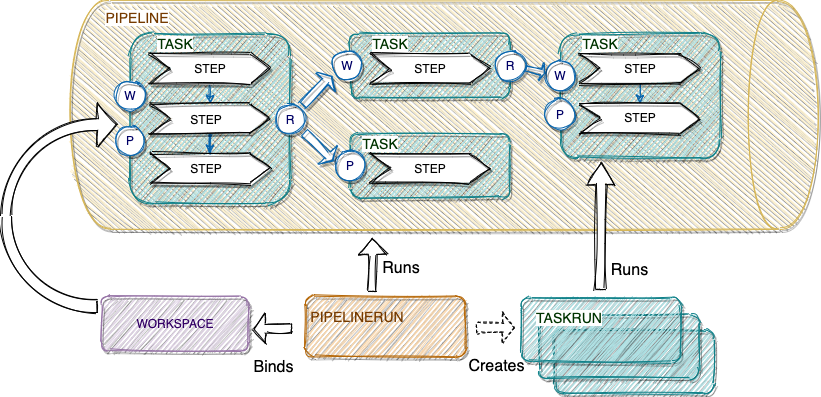
\includegraphics[width=0.5\paperwidth]{img/tekton-workspaces.png}
  \end{textblock*}
  % Knative, Tekton and the CDF
\end{lgrayrwhiteframe}

\note{
  Focus on extending the k8s API.
  New resources / abstraction to build and run your pipelines
}

\section[Authoring]{Authoring}

\begin{sectionwithpicrx}[pierre-bamin--ltjzTfhpCI-unsplash.jpg]{Photo by \href{https://unsplash.com/@bamin}{\underline{Pierre Bamin}}, CC0}
\end{sectionwithpicrx}

\begin{lpicrblack}[antoine-petitteville-RIdYHUISNuM-unsplash.jpg]{%
  Photo by \href{https://unsplash.com/@ant0ine}{\underline{Antoine Petitteville}}, CC0
  }%
  {%
    Steps:
    \begin{itemize}
      \item Off the Shelves containers
      \item Small scripts % no large scripts in YAML!
    \end{itemize}
    Tasks:
    \begin{itemize}
      \item Solve one specific problem
      \item Owned by a team
      \item Distributed maintenance
    \end{itemize}
    \vspace{0.05\paperheight}
    Reusability:
    \begin{itemize}
      \item Discovery
      \item Versioning
      \item Best Practices
    \end{itemize}
  }{}%
  \frametitle{Building Blocks}
\end{lpicrblack}

\note{
  Scalable authoring depends on reusability and maintainability
  Teams need to be able to use tasks and pipelines and connect them
  as lego blocks. Task and pipeline maintaners need to be able to
  build new versions of tasks without breaking downstream users.
}

\begin{grayframe}
  \frametitle{Catalog and Hub}
  Discovery:
  \begin{itemize}
    \item Kubernetes cluster
    \item Tekton Catalog
    \item Tekton Hub \& API
  \end{itemize}
  \vspace{0.03\paperheight}
  Versioning:
  \begin{itemize}
    \item Tekton Bundles
    \item \texttt{tkn bundle [push|list]}
    \item \texttt{gcr.io/tekton-releases/catalog/upstream/}
  \end{itemize}
  \vspace{0.03\paperheight}
  Best Practices:
  \begin{itemize}
    \item Params, Results, Workspaces % Good defaults, optional when possible
    \item Portability % multi-arch images
  \end{itemize}
  % open source, small team, authoring efficiency is important
  % IBM, migrating customers to Tekton, large number of tasks
  \begin{textblock*}{0.4\paperwidth}(0.42\paperwidth,0.05\paperheight)
    \begin{tikzpicture}%
      \node [opacity=0.9]{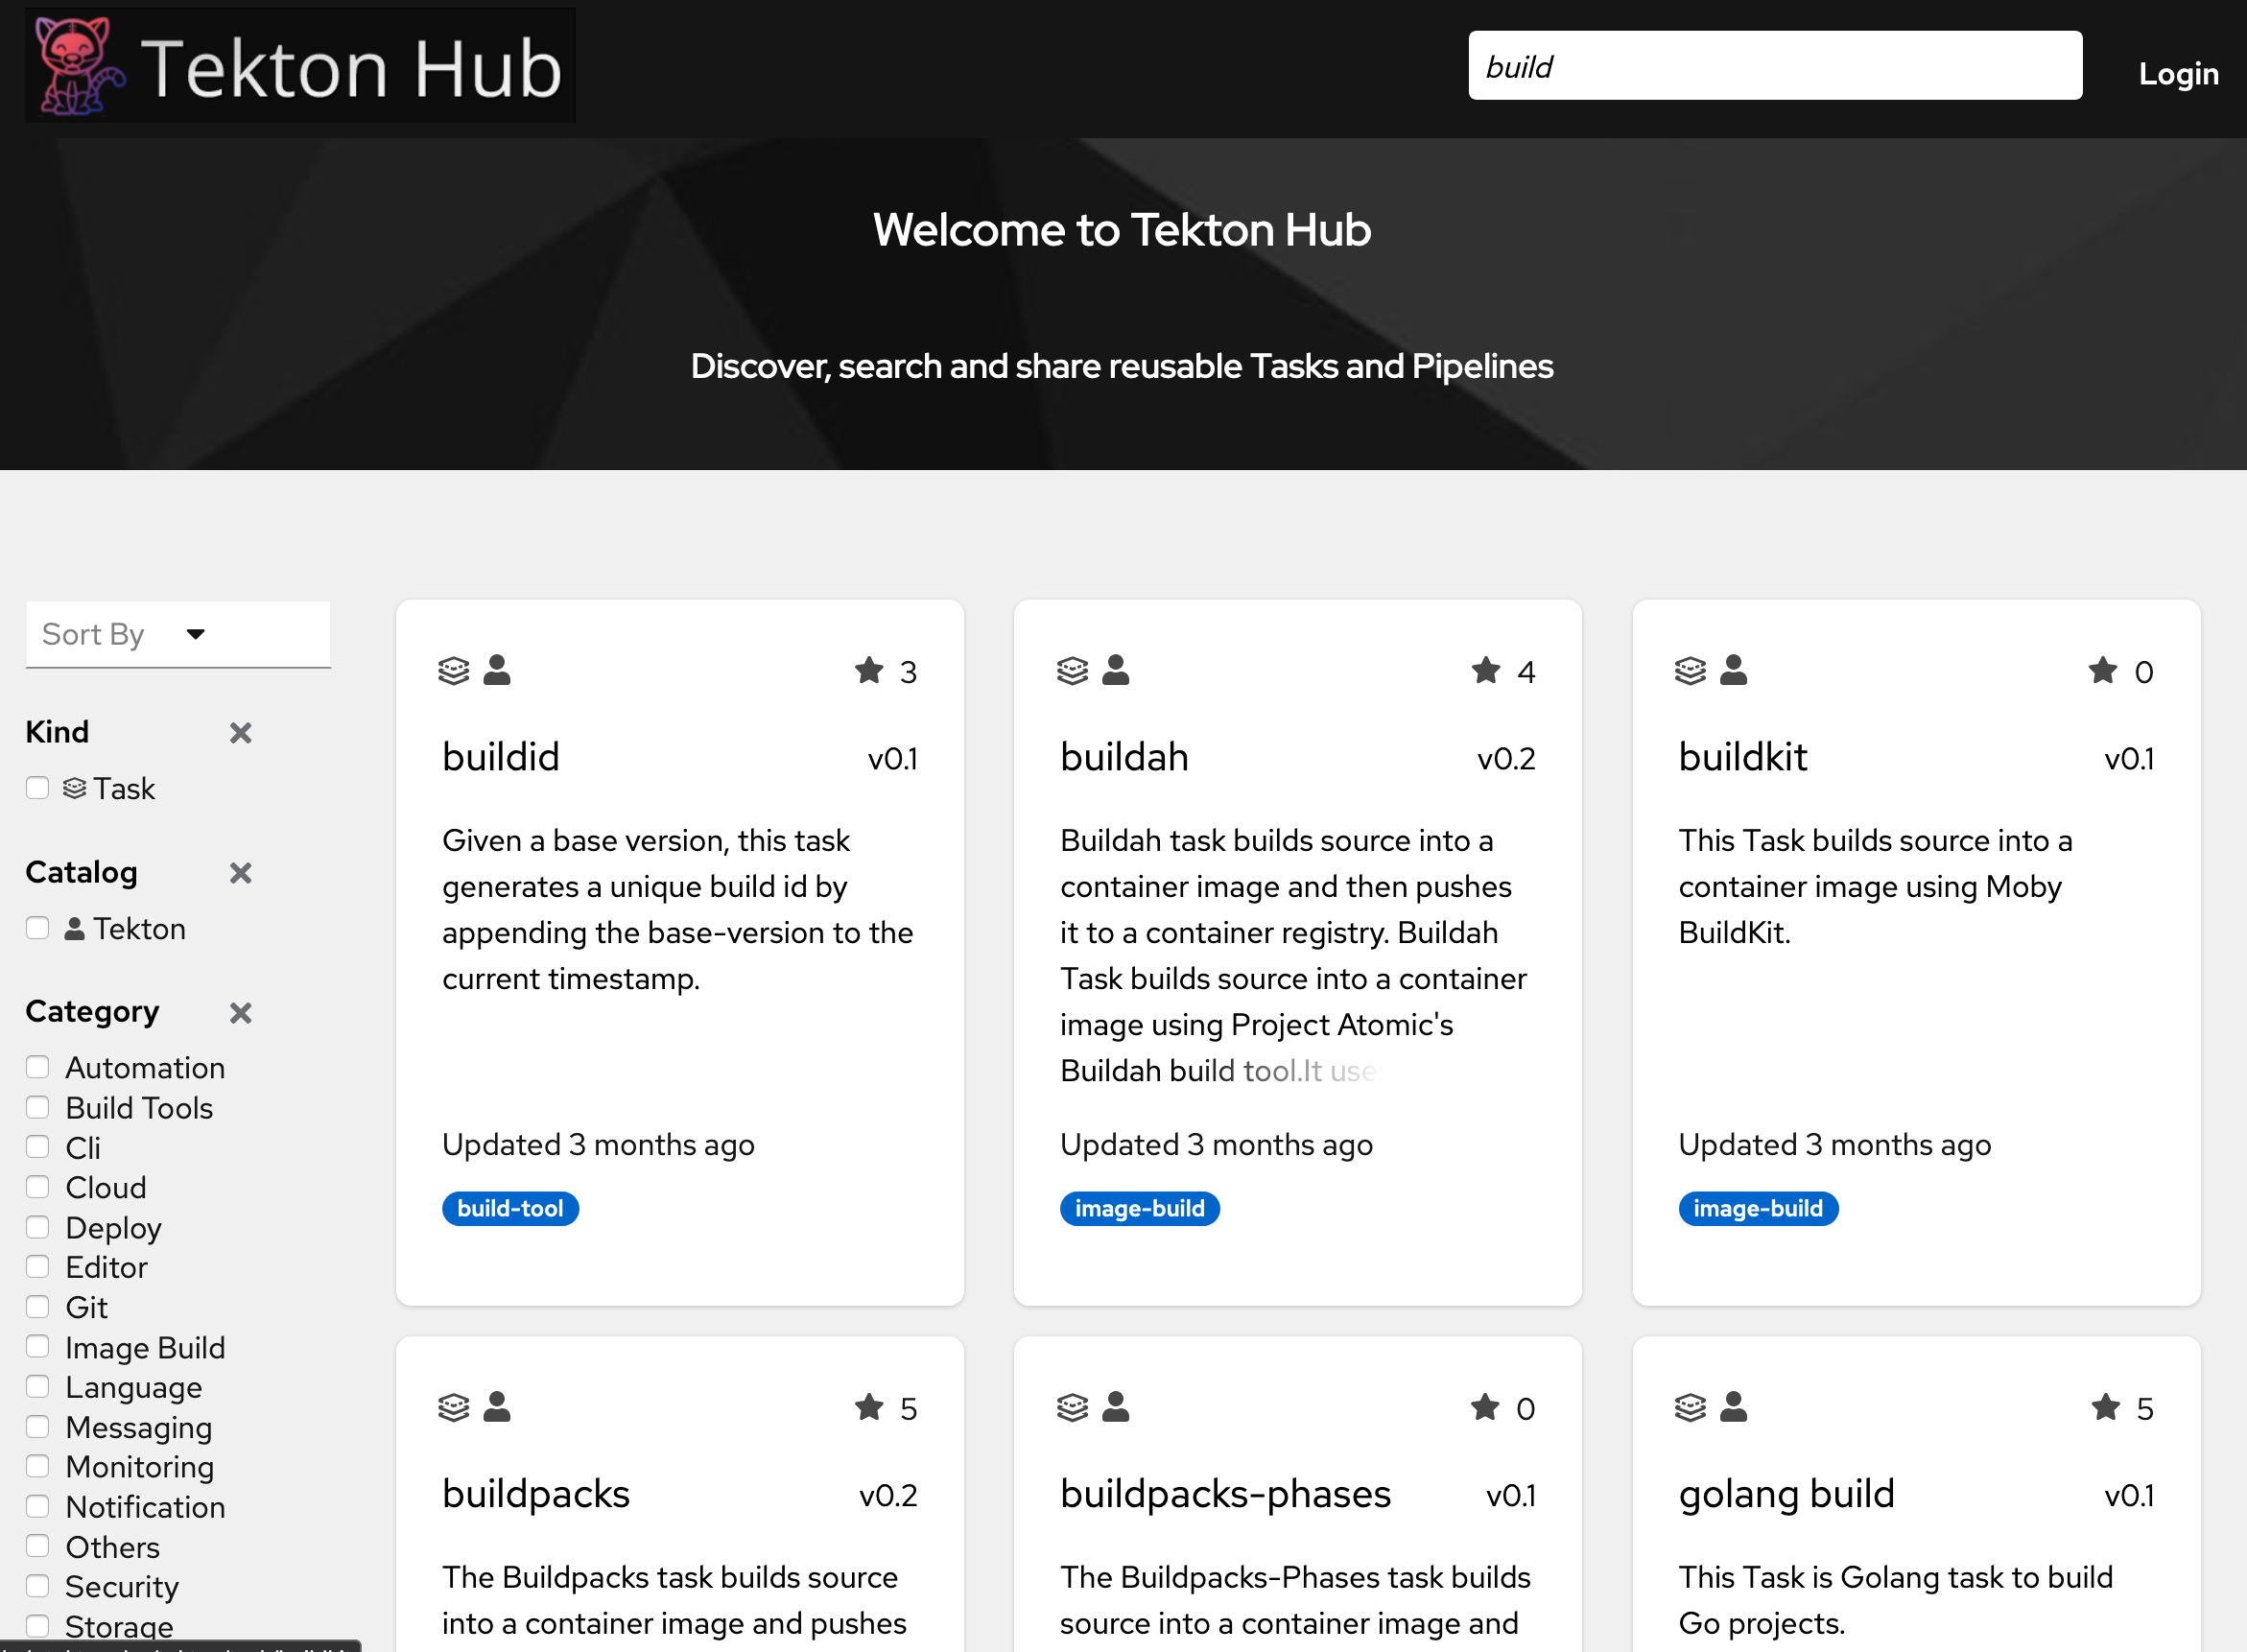
\includegraphics[width=0.4\paperwidth]{img/hub.png}};%
    \end{tikzpicture}
  \end{textblock*}
  \begin{textblock*}{0.3\paperwidth}(0.63\paperwidth,0.45\paperheight)
    \begin{tikzpicture}%
      \node [opacity=0.8]{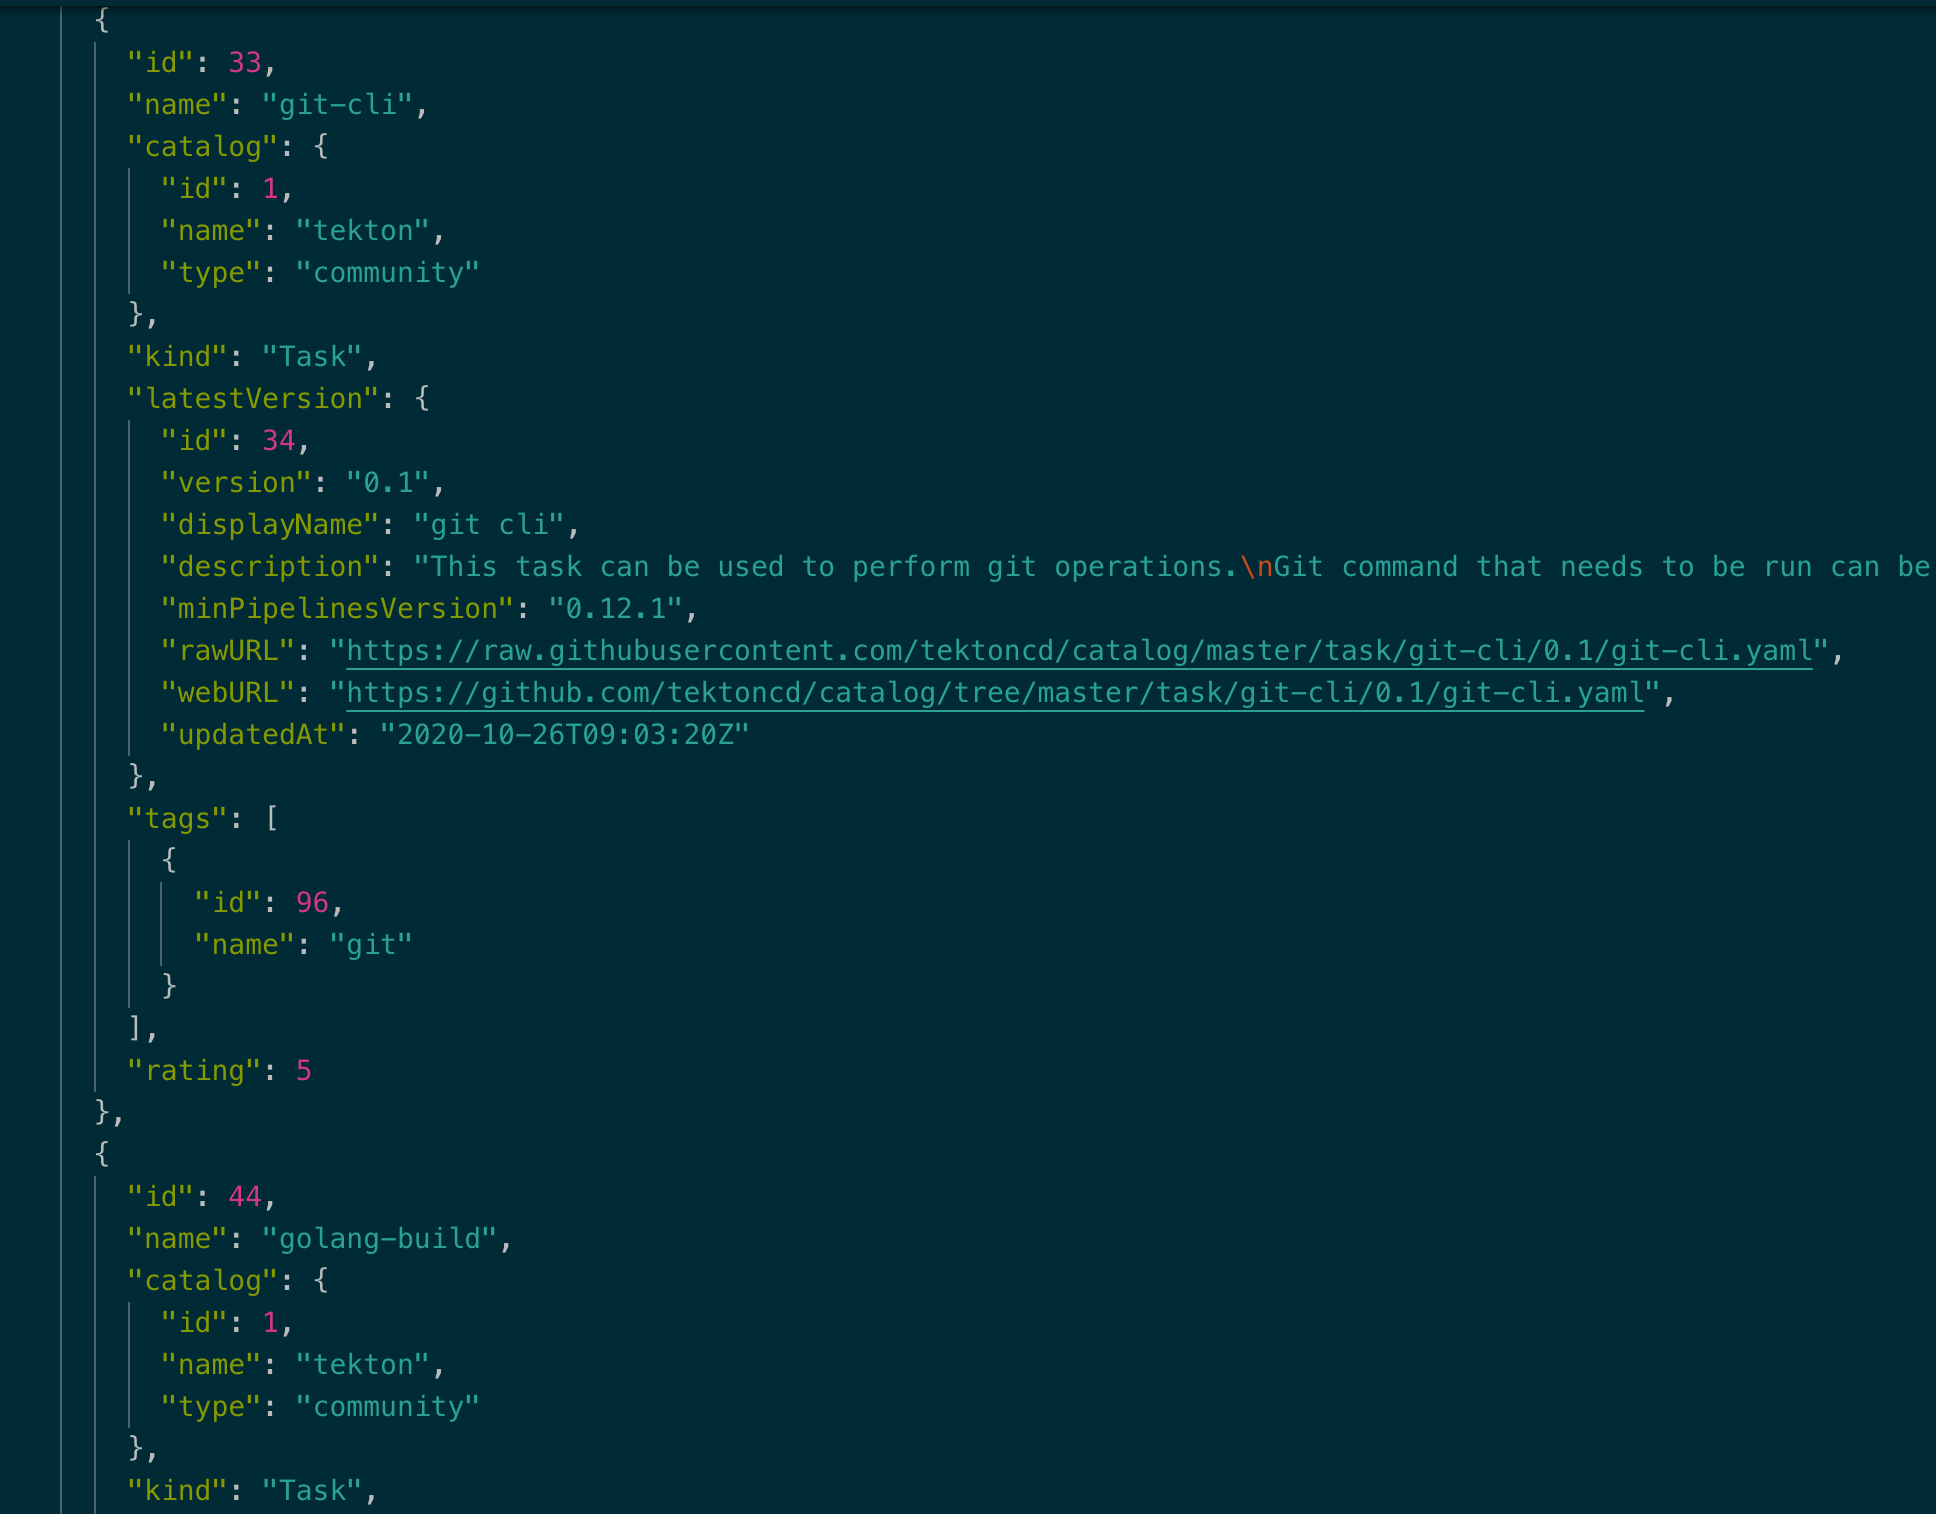
\includegraphics[width=0.3\paperwidth]{img/hub-api.png}};%
    \end{tikzpicture}
  \end{textblock*}
  % Sharing Tasks and discovery
  % Tekton Bundles
\end{grayframe}

\note{
  Reusability!!!
  Add a short demo:
  - Search and install a task with tkn
  - Create a task from a local YAML
  - Put them together as a pipeline
  - Push the local task to an OCI bundle
  - Re-run the pipeline with bundles
  Talk about how orgs can build their own catalog(s)
  Share their tasks through bundles
}

\begin{tpicstripedframe}%
  {tekton-pipeline-blocks.png}%
  {%
  Short pipelines: \\
  \vspace{0.03\paperheight}
  Building blocks
  \begin{itemize}
    \item Conditions
    \item Optional Inputs
  \end{itemize}
  }%
  {%
  Large Pipelines:
  \vspace{0.03\paperheight}
  How to:
  \small
  \begin{itemize}
    \item Add a Branch \\
    \item Swap a Block \\
    \item Access Control \\
    \item Distribute \\
  \end{itemize}
  }%
  {%
  Distribute:
  \vspace{0.03\paperheight}
  \begin{itemize}
    \item Team
    \item Access
    \item Namespace
    \item Cluster
    \item Platform
  \end{itemize}
  }%
  {%
  One workflow: \\
  \vspace{0.03\paperheight}
  \begin{itemize}
    \item Pipeline in Pipeline (experimental)
    \item \texttt{CloudEvents}
  \end{itemize}
  }%
  \frametitle{Pipelines}
  % Example: clone, build, scan, push, test, release, e2e test, publish \\
  % Supported by the catalog. \\
  % What scan strategy? Which tests? \\
  % I could have multiple test pipelines \\
  % Different parts owned by different teams \\
  % We still need small pipelines to do one job \\
  % How do I connect them?
  % Ever growing pipeline, multiple teams add to it
\end{tpicstripedframe}

\section[Running]{Running}

\begin{sectionwithpic}[pexels-ray-bilcliff-1509237.jpg]{Photo by \href{https://www.pexels.com/@raybilcliff}{\underline{Ray Bilcliff}}, CC0}
\end{sectionwithpic}

\begin{lgrayrwhiteframe}
  \frametitle{Triggers}
  Run Pipelines on Events:
  \begin{itemize}
    \item HTTP POST
    \item Pull Request, Image Published
  \end{itemize}
  \vspace{0.02\paperheight}
  Components:
  \begin{itemize}
    \item Receive: Event Listener
    \item Filter: Interceptors
    \item Run: Binding and Templates
  \end{itemize}
  \vspace{0.02\paperheight}
  Generate Events:
  \begin{itemize}
    \item k8s and CloudEvents
    \item Start, Run and Stop
  \end{itemize}
  \begin{textblock*}{0.51\paperwidth}(0.48\paperwidth,0.33\paperheight)
    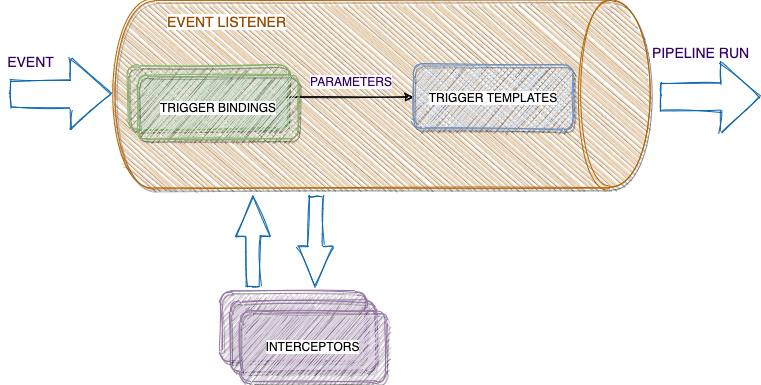
\includegraphics[width=0.5\paperwidth]{img/tekton-triggers.png}
  \end{textblock*}
\end{lgrayrwhiteframe}

\begin{tpicstripedframe}%
  {tekton-pipeline-async.png}%
  {%
  Receiving and sending events \\
  \vspace{0.03\paperheight}
  Composite Workflow \\
  \vspace{0.03\paperheight}
  Separate Ownership \\
  }%
  {%
  Dynamically add tasks \\
  \vspace{0.03\paperheight}
  Reuse pipeline \\
  \vspace{0.03\paperheight}
  Heterogeneous parts
  }%
  {%
  \textit{Issues}: \\
  \vspace{0.03\paperheight}
  Custom integrations \\
  \vspace{0.03\paperheight}
  Orchestration \\
  Visibility
  \vspace{0.03\paperheight}
  }%
  {%
  Events in CI/CD Special Interest Group \\
  \vspace{0.05\paperheight}
  \centering
  \includesvg[width=0.1\paperwidth]{img/cdf-icon-white.svg}
  }%
  \frametitle{Events}
  % Receiving and sending events
  % Further spread responsibility, break the pipeline
  % Interop and event SIG
\end{tpicstripedframe}

\section[Bottlenecks]{Bottlenecks}
\begin{sectionwithpicrx}[dan-cristian-padure-LDMgqr8z7ZE-unsplash.jpg]{Photo by \href{https://unsplash.com/@dancristianp}{\underline{Dan-Cristian Pădureț}}, CC0}
\end{sectionwithpicrx}

{
\begin{tblackbgrayframe}{Very Large pipelines}
  %\frametitle{Growing pipelines}
  \begin{itemize}
    \item Directed Acyclic Graphs
    \item Large Pipelines (100 nodes, densely connected)
    \item Scale Issues?
  \end{itemize}
  \begin{itemize}
    \item DAG build on every reconcile
    \item Hundreds of nodes and connections
    \item Optimized code in the DAG computation
  \end{itemize}
  \begin{itemize}
    \item Maintainability
    \item Pod Overhead
  \end{itemize}
  \begin{textblock*}{0.42\paperwidth}(0.55\paperwidth,0.35\paperheight)
    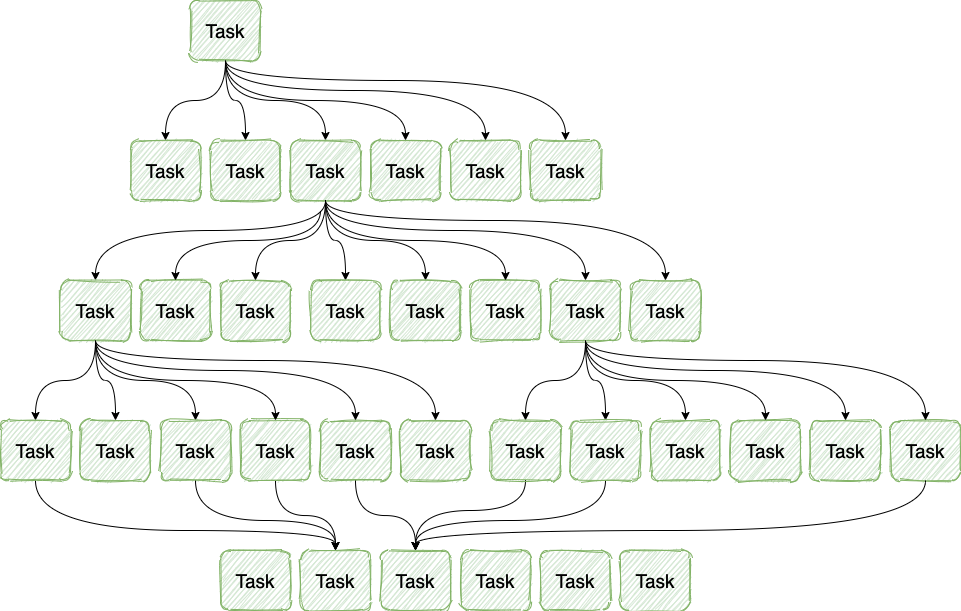
\includegraphics[width=0.42\paperwidth]{img/tekton-large-dag.png}
  \end{textblock*}
\end{tblackbgrayframe}
}

\begin{2columnsframe}%
  {%
    Under Pressure - Running \textbf{many} Pipelines%
  }%
  {%
  Concurrent execution
  \begin{itemize}
    \item Cached K8s API calls: Informers
    \item Scale Up Controllers: LeaderElection
    \item Cluster Resources: K8s scheduler
  \end{itemize}
  \vspace{0.17\textheight}
  Potential enhancements:
  \begin{itemize}
    \item Throttling pipeline execution
    \item Optimize Execution Runtime
    \item Tekton custom scheduler
  \end{itemize}
  }%
  {%
  In real life
  \begin{itemize}
    \item Thousands Tasks/month upstream
    \item Millions containers/month @IBM
    \item Throttling (for security too)
  \end{itemize}
  \vspace{0.17\textheight}
  Cluster pollution?
  \begin{itemize}
    \item Tekton Results
  \end{itemize}
  }
\end{2columnsframe}

\section[Roadmap]{Conclusions \& Roadmap}
\begin{sectionwithpich}[julie_falk_flickr_22258190324_6a583208ae_k.png]{Photo by \href{https://www.flickr.com/photos/piper/}{\underline{Julie Falk}}, CC BY-NC 2.0}
\end{sectionwithpich}

\begin{lpicrblack}[john-yunker-Z9rKuPEU6Uc-unsplash.jpg]{%
  Photo by \href{https://unsplash.com/@jyunker}{\underline{John Yunker}}, CC0
  }%
  {%
    Author Time Scalability:
    \begin{itemize}
      \item Best Practices
      \item Reusable Tasks and Pipelines
      \item Versioning \& Sharing
      \item Break Down Large Pipelines
     \end{itemize}
    \vspace{0.1\paperheight}
    Run Time Scalability:
    \begin{itemize}
      \item Cloud Native \& Scalable
      \item Execution Throttling
      \item Pod execution overhead
    \end{itemize}
    \vspace{0.01\paperheight}
  }{}%
  \frametitle{}
\end{lpicrblack}

{
\begin{tblackbgrayframe}{Roadmap}
  %\frametitle{Growing pipelines}
  \begin{itemize}
    \item Continue Dogfooding Tekton at Scale!
    \item Pipelines in Pipelines \href{https://github.com/tektoncd/community/blob/main/teps/0056-pipelines-in-pipelines.md}{TEP-0056}
    \item Remote Resource Resolution \href{https://github.com/tektoncd/community/blob/main/teps/0060-remote-resource-resolution.md}{TEP-0060}
    \item Decouple Task Composition from Scheduling \href{https://github.com/tektoncd/community/blob/main/teps/0044-decouple-task-composition-from-scheduling.md}{TEP-0044}
    \item Runtime Task Bundle Definitions \href{https://github.com/tektoncd/community/pull/429}{TEP-0068}
    \item Implement the SIG Events format of Cloud Events
  \end{itemize}
  \begin{textblock*}{0.28\paperwidth}(0.65\paperwidth,0.35\paperheight)
    
\includegraphics[width=0.28\paperwidth]{img/tekton-icon-color.png}
  \end{textblock*}
\end{tblackbgrayframe}
}

\section[Q\&A]{Thank You! \\Questions?}

\begin{sectionwithpiclargecentral}[carl-jorgensen-5nrnxx_tWe8-unsplash.jpg]{Brecon Beacons, Walse, Photo by \href{https://unsplash.com/@scamartist}{\underline{Carl Jorgensen}}, CC0}
\end{sectionwithpiclargecentral}

\begin{blackframe}
  \frametitle{References}
  \begin{itemize}
    \item \large Come and Join Us at Tekton!
    \item \normalsize Tekton community: \href{https://github.com/tektoncd/community}{github.com/tektoncd/community} \\
  \end{itemize}
  \begin{itemize}
    \item Slides: \href{https://github.com/afrittoli/scaling_pipelines_with_tekton/blob/cdcon2021/scaling_pipelines_with_tekton.pdf}{github.com/afrittoli/scaling\_pipelines\_with\_tekton}
    \item Tekton: \href{https://tekton.dev}{tekton.dev}
    \item Tekton on GitHub: \href{https://github.com/tektoncd}{github.com/tektoncd}
    \item Tekton Results: \href{https://github.com/tektoncd/results}{github.com/tektoncd/results}
    \item Tekton Hub: \href{https://hub.tekton.dev}{hub.tekton.dev}
    \item Tekton TEPs: \href{https://github.com/tektoncd/community/tree/main/teps}{github.com/tektoncd/community/tree/main/teps}
  \end{itemize}
  \begin{textblock*}{0.13\paperwidth}(0.73\paperwidth,0.65\paperheight)
    \includesvg[width=0.13\paperwidth]{img/tekton-icon-color.svg}
  \end{textblock*}
\end{blackframe}

\end{document}
